\newpage
\section{Power Sensor}
The purpose of this block is to measure the electrical power delivered to the car's propulsion system. The power sensor must be able to measure both the delivered voltage V and  current I, as the power P is given by:
\begin{equation}
	P = V \cdot I
\end{equation}

\subsection{Design}
The design is split in two due to the fact that the sensor must measure two parameters.

\textbf{Current Transducer}\\
The current is measured using a Hall-effect based current transducer of the type LTS 15-NP. The internal circuit of the component is seen on Figure \ref{fig:LTS_internal_circuit} below. The transucer measures the strength of the magnetic field induced by the input current and converts it to a voltage. This voltage is amplified and given as the transducer's output. The internal amplifier must be supplied with 5 VDC in order for the transducer to measure properly.

\begin{figure}[H]
	\centering
	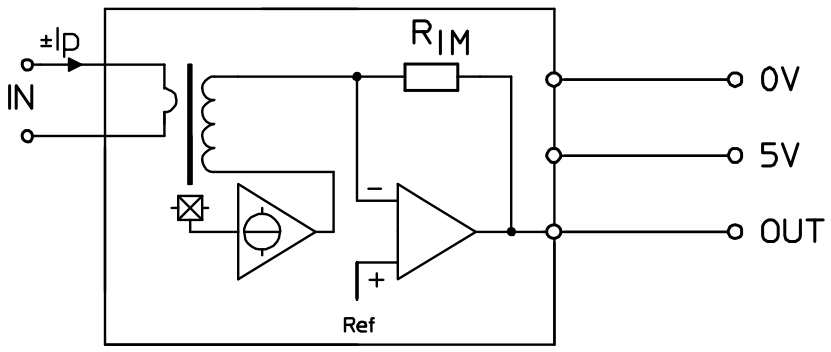
\includegraphics[width=0.5\linewidth]{Hardware/Pictures/LTS_circuit}
	\caption{LTS 15-NP Internal circuit}
	\label{fig:LTS_internal_circuit}
\end{figure}

The LTS 15-NP is gives an output-voltage which is proportional to the input-current and lies in the range between $\SI{0.5}{\volt}$ and $\SI{4.5}{\volt}$. The transducer contains 6 pins which can be connected in different ways in order to change the number of primary turns in the coil - and thus changing the primary nominal current rms I\textsubscript{PN}. This means that the input's measuring range can be configured as the output-voltage V\textsubscript{out} can be described using the following formula:
\begin{equation}
	V_{out} = 2.5 \pm \left( 0.625 \cdot \frac{I_{P}}{I_{PN}} \right)
	\label{eq:current_transducer}
\end{equation}

Where I\textsubscript{P} is the transducer's input current. The formula above can be used to plot the output on Figure \ref{fig:LTS_output} below. The accuracy of the transducer is specified to 0.2\%.

\begin{figure}[H]
	\centering
	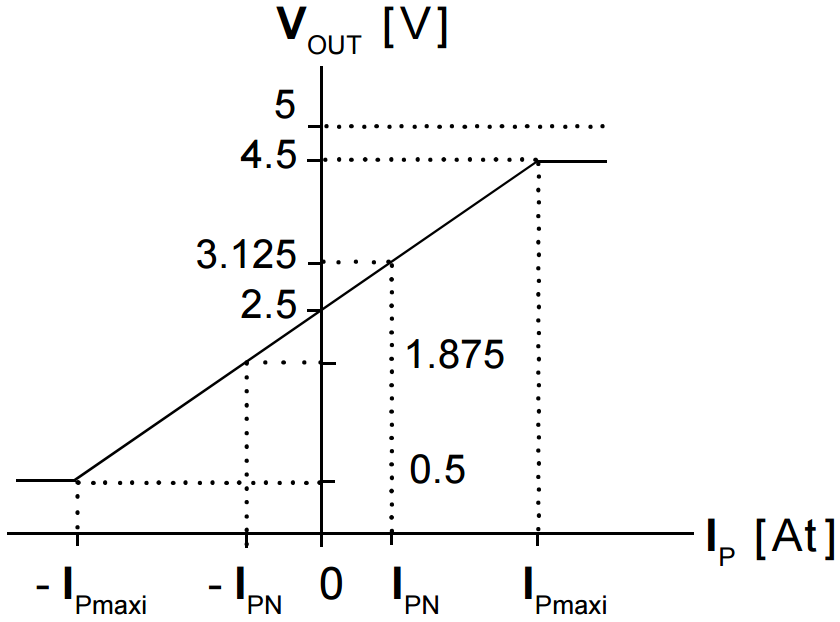
\includegraphics[width=0.4\linewidth]{Hardware/Pictures/LTS_output}
	\caption{LTS 15-NP Output voltage}
	\label{fig:LTS_output}
\end{figure}

The transducer's pins are configured in such a way that the the primary nominal current rms I\textsubscript{PN} is equal to $\pm \SI{15}{\ampere}$. This allows for the largest measuring range possible. Using this number and equation \ref{eq:current_transducer} it is possible to calculate the range wherein the transducer measurements are linear.

The minimum-current which the transducer can measure correctly before it enters saturation can be calculated as:
\begin{equation}
	0.5 = 2.5 + \left( 0.625 \cdot \frac{I_{Pmini}}{15} \right) \quad \Rightarrow \quad I_{Pmini} = \SI{48}{\ampere}
\end{equation}

The maximum-current which the transducer can measure correctly before it enters saturation can be calculated as:
\begin{equation}
	4.5 = 2.5 + \left( 0.625 \cdot \frac{I_{Pmaxi}}{15} \right) \quad \Rightarrow \quad I_{Pmaxi} = \SI{-48}{\ampere}
\end{equation}

The transducer's measuring-resolution can be calculated as a output-difference per the corrosponding input-difference. The difference is found using the minimum and maximum range values from the calculations above:
\begin{equation}
	\Delta V = \frac{\SI{4.5}{\volt} - \SI{0.5}{\volt}}{\SI{48}{\ampere} - (\SI{-48}{\ampere})} = \SI[per-mode = fraction]{41.67}{\milli \volt \per \ampere}
\end{equation}

\textbf{Voltage Transducer}\\
The voltage delivered to the motor is measured using a voltage divider consisting of two resistors. The voltage didiver must be placed parallel to the motor to correctly measure the voltage.

\subsection{Implementation}
Text

\subsection{Unity test}
Text